\documentclass[a4paper]{article}
\usepackage{geometry}
\geometry{left=3.5cm,right=3.5cm,top=3.5cm,bottom=3.5cm}
\usepackage{amsmath, amssymb}
\usepackage{graphicx}
\usepackage{subfigure}
\usepackage{pdfpages}

\usepackage{xeCJK}
\setmainfont{Times New Roman}
\setCJKmainfont[BoldFont=SimHei,ItalicFont=KaiTi]{SimSun}

\usepackage{indentfirst}
\setlength{\parindent}{2em}

\usepackage{fancyhdr}
\pagestyle{fancy}
\usepackage{lastpage}
\rhead{}
\lhead{}
\cfoot{\thepage{}}
\renewcommand{\headrulewidth}{0pt}
\renewcommand{\figurename}{图}
\renewcommand{\tablename}{表}
\renewcommand{\abstractname}{摘要}
\renewcommand{\contentsname}{\CJKfamily{SimHei} 目录}

\headheight 14pt

\usepackage{float}

\renewcommand\baselinestretch{1.2}

\begin{document}

\begin{titlepage}

\includepdf[pages=3-4,offset=0cm 0cm]{title.pdf}

\end{titlepage}

\begin{Huge}
	\textbf{\centerline{ATM 交易状态特征分析与异常检测}}
\end{Huge}
\begin{large}
	\begin{flushright}
		
	\end{flushright}
\end{large}
\ \ \\\\

\begin{abstract}
\textit{}
\end{abstract}

\newpage

\tableofcontents

\newpage

\part{引言}
近些年来,由于人民生活水平的提高,银行的业务量飞速提升。与此同时也带了取款存款难的问题。为了解决这个问题,近几年许多银行都开始广泛使用ATM自动取款机,并建立了一套ATM交易系统。在银行的ATM交易系统中,银行总行数据中心监控系统为了实时掌握全行的业务状态,每分钟会对各分行的交易信息进行汇总统计。汇总信息包括业务量、交易成功率、交易响应时间三个指标。监控系统要从这三个指标的变化情况中及时发现ATM交易系统是否出现故障。

\part{表征交易状态的特征参量}
\chapter{业务量的特征参数}
\chapter{成功率的特征参数}
\chapter{响应时间的特征参数}

\part{交易状态异常检测方案}
\chapter{基于ICA算法的含噪声时间序列预测}
\chapter{与其他方法的比较分析}
\chapter{对方案可靠性的评估}
\chapter{不同突变点原因分析}

\part{方案的优化及完善}

\end{document}
